% page number: less or equal to 15
Un modello matematico serve a rappresentare e a fornire previsioni sullo stato
futuro di un fenomeno o di un sistema. Il modello, quindi, descrive la probabile
evoluzione di un fenomeno o di un sistema sulla base di dati di ingresso,
forniti dall'utente e restituendo dei dati di uscita, che andranno poi
confrontati con i dati di uscita previsti, per valutare l'efficacia del modello.
Nel nostro caso, quello di un satellite in orbita attorno alla terra,
l'efficacia del modello è di estrema importanza, perché piccoli errori
potrebbero causare la perdita del satellite e quindi di ingenti somme di denaro
e lavoro spesi per realizzarlo. In questo capitolo verra trattata la
modellazione della dinamica dell'orbita e il calcolo della dinamica e della
cinematica dell'assetto del satellite.
\begin{section}{Orbit dynamics}
%###
\subsection{Equations(two bodies motion)}
Consideriamo un sistema costituito da due corpi puntiformi $P_0$ e
$P_1$ aventi ripettivamente massa $m_0$ e $m_1$, definiamo la loro posizione e
velocità rispetto a un sistema inerziale $\mathfrak{R} \{
O,\bar{i_1},\bar{i_2},\bar{i_3}\}$, siano quindi $r_0$ e $r_1$ le posizioni e
$v_0$ e $v_1$ le velocità dei due corpi. Dalla seconda legge di Newton,
ricaviamo:
\begin{equation}
\begin{array}{l}
\dot{v_0}(t)=\frac{Gm_0m_1}{m_0r^3}r(t) + \frac{1}{m_0}F_0(t),v_0(0)=v_{00}\\\\
\dot{v_1}(t)=\frac{Gm_0m_1}{m_1r^3}r(t) + \frac{1}{m_1}F_1(t),v_1(0)=v_{10}
\end{array}
\end{equation}
dove: $r(t)=r_1(t)-r_0(t)$, $G=66.7x10^{-12} m^3kg^{-1}s^{-2}$ è la costante di
gravitazionale universale, mentre $F_0(t)$ e $F_1(t)$ sono due forze esterne
agenti sui corpi.
Studiamo il sistema nel suo insieme, quindi, sia $r_c$ il centro di massa del
sistema costituito dai due corpi, la sua accelerazione $\dot{v_c}$ risulta essere:
\[r_c=\frac{m_0}{m_0+m_1}r_0+\frac{m_1}{m_0+m_1}\]
\begin{equation}
\dot{v}(t)=\dot{v_1}(t)-\dot{v_0}(t)=-\frac{G(m_0+m_1)}{r^3}r(t)+\frac{1}{m_1}(F_1(t)-\frac{m_1}{m_0}F_0(t)),
v(0)=v_0
\end{equation}
\begin{equation}
\dot{v_c}(t)=\frac{F_1(t)+F_0(t)}{m_0+m_1},v_c(0)=v_{c0}
\end{equation}
Nel nostro caso il sistema è costituito dalla Terra e dal satellite in orbita
attorno ad essa. Poiché la massa della Terra è molto maggiore rispetto quella
del satellite, $m_0>>m_1$ le equazioni diventano:
\begin{equation}
\dot{v}(t)=-\frac{\mu_0}{r^3}r(t)+\frac{F_1(t)}{m_1}, v(0)=v_0
\label{eq:2body_acc}
\end{equation}
\begin{equation}
\dot{v_c}(t)=0, v_c(0)=v_{c0}
\end{equation}
dove $\mu_0=Gm_0$.
Il centro di massa $r_c$ lo si può approssimare al centro di massa della Terra
e, poiché la sua accelerazione è nulla, possiamo considera un sistema di
riferimento centrato in esso. L'equazione \ref{eq:2body_acc} riscritta
nel nuovo sistema di riferimento è nota come equazione ristretta del problema
dei due corpi.

\subsection{Orbit Parameters} 
Per conoscere i parametri orbitali dobbiamo prima calcolare la risposta libera
del nostro sistema. Riscriviamo l'equazione $\ref{eq:2body_acc}$ senza
considerare le forze esterne
\begin{equation}
\dot{\bf v}(t)=-\frac{\mu_0}{r^3}{\bf r(t)}, v(0)=v_0
\end{equation}
La risposta libera descrive un'orbita che giace su un piano fisso, il piano
orbitale, definito dai vettori velocità e posizione. Si nota che l'accelerazione
è istante per istante opposta al vettore posizione, quindi se prendiamo in esame
il momento angolare per unità di massa {\bf h(t)}, definito come ${\bf
h(t)}={\bf r(t)}$ x ${\bf v(t)}$, la sua derivata è uguale a zero. Quindi ${\bf
h}=h{\bf e_h}$ è un vettore costante in direzione ${\bf e_h}$ (il polo dell'orbita) e
magnitudine h, che può essere presa come asse del sistema di riferimento.
Mediante il momento angolare possiamo anche definire il vettore eccentricità
\begin{equation}
{\bf v}(t) \times {\bf h} - \frac{\mu}{r(t)}{\bf r}(t)=\mu{\bf e}
\label{eq:eccentricity}
\end{equation}
$e=|{\bf e}|$ rappresenta  l'eccentricità dell'orbita e la sua direzione
l'origine della risposta libera. La forma dell'orbita dipende dalla sua
eccentricità, esistono tre tipi di coniche in funzione del valore di $e$
\begin{itemize}
  \item ellisse per $e<1$, che diventa una circonferenza quando e=0
  \item parabola per e=1 
  \item iperbole per $e>1$
\end{itemize}
Moltiplicando scalarmente per {\bf r(t)} l'equazione \ref{eq:eccentricity} si ottiene l'equazione
della risposta libera
\begin{equation}
h^2(t)-\mu r(t)=\mu r(t)e \cos{\theta(t)}
\label{eq:free_response}
\end{equation}
$\theta$, che rappresenta l'angolo tra $r$ ed $e$, è detto anomalia vera.
Riscrivendo l'equazione \ref{eq:free_response} in funzione del raggio orbitale,
otteniamo
\begin{equation}
r(t)=\frac{p}{1+e\cos{\theta{t}}} , p=\frac{h^2}{\mu}
\end{equation}
La costante p[m] è definita semilatus rectum. In figura \ref{fig:LVLH} è mostrata la
geometria del'orbita nel sistema di riferimento Local Vertical Local Horizontal (LVLH)
$\mathfrak{R_l}$=$\mathfrak{R}=\{C,\bar{l_1},\bar{l_2}=e_h,\bar{l_3}\}$ dove
$\bar{l_3}=\bar{e_r}=\bar{r}/r$ definisce la verticale locale, $l_1=e_{\theta}$
la orizzontale locale e $l_2=e_h$ è il polo orbitale.

\begin{figure}[htp]
\begin{center}
  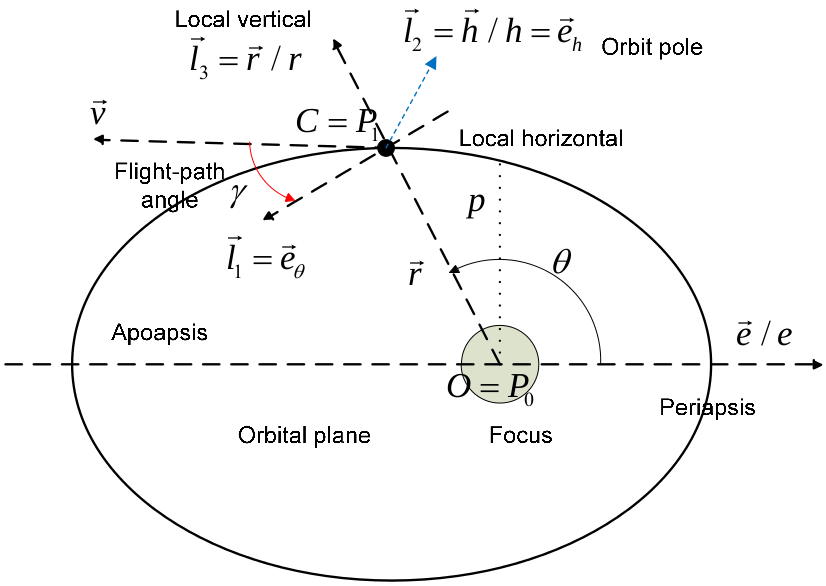
\includegraphics[width=\textwidth]{modelling/orbit_dynamics/image/LVLH.png}
  \caption{Geometria dell'orbita e sistema di riferimento LVLH}
  \label{fig:LVLH}
\end{center}
\end{figure}
Introduciamo il parametro $a$, che definisce il semi-asse maggiore dell'orbita
ellittica, e l'anomalia eccentrica $E$, il quale rappresenta l'angolo tra la
linea degli absidi e la linea tra $C_0$ , centro dell’ellisse, e $Q_1$ ,
definito come la proiezione del punto $P_1$ su un cerchio ausiliario di centro
$C_0$ come illustrato in figura \ref{fig:cerchio_ausiliario}.
\begin{figure}[htp]
\begin{center}
  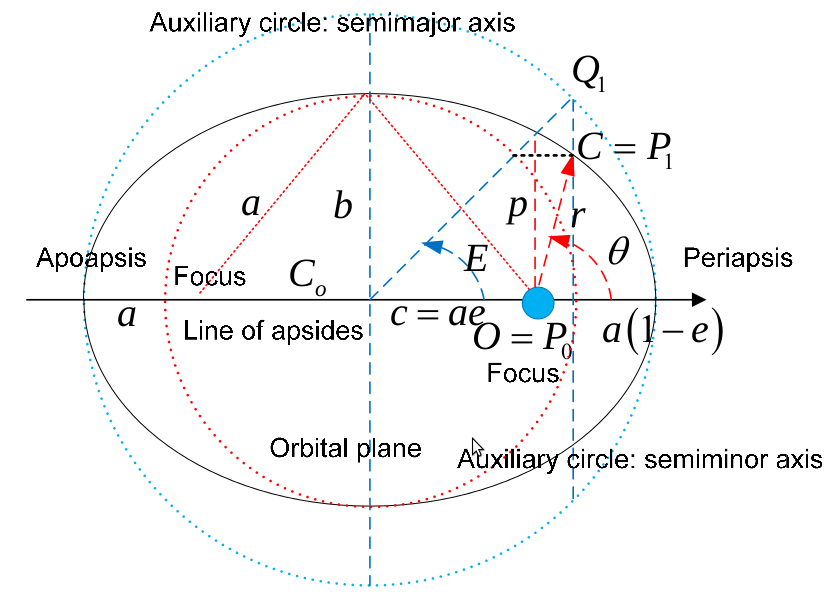
\includegraphics[width=\textwidth]{modelling/orbit_dynamics/image/cerchio_ausiliario.png}
  \caption{Geometria dell'orbita ellittica e cerchio ausiliario}
  \label{fig:cerchio_ausiliario}
\end{center}
\end{figure}

Per effettuare le simulazioni in ambiente Matlab è necessario introdurre
ulteriori parametri
\subsection{Free response simulation}
La risposta libera la si calcola azzerando le forze esterne, così facendo
otteniamo l'equazione \ref{eq:free_response}
\begin{equation}
\dot{\bf v}(t)=-\frac{\mu_0}{r^3}{\bf r(t)}, v(0)=v_0 \nonumber
\end{equation}
Per poter simulare l'andamento del satellite in risposta libera, dobbiamo
eliminare tutti i disturbi esterni, come ad esempio il drag, la costante $J_2$
(essa è definita come la seconda armonica zonale e rappresenta l'appiattimento
ai poli del globo terrestre), inoltre bosogna annullare il controllo e spegnere
i propulsori. L'unica forza esterna sarà quella gravitazionale del pianeta
Terra, ma, per rendere la simulazione più ideale, la consideriamo sferica. Per
fare ciò in Matlab impostiamo i seguenti parametri:
\begin{lstlisting}[language=matlab,breaklines=true]
GravityTypeFlag=0;		%(1=J2 Gravity Model/=0 Spherical)
GravityGradientTorqueFlag=0;	%1=Gravity Gradient Torque ON/0=OFF 
DragForceDisturbancesFlag=0;	%0=Drag Force Disturbance OFF/1=OFF
DragTorquesDisturbancesFlag=0;	%0=Drag Torque Disturbance OFF/1=ON
DragFreeControlFlag=0;		%0=Drag Free Control OFF/1=ON
AttitudeControlFlag=0;		%0=Attitude Control OFF/1=ON
\end{lstlisting}
\subsection{Perturbations}
%###
\end{section}
\begin{section}{Attitude kinematics and dynamics}
%###
\subsection{Equations}
L'assetto (o orientamento) di un corpo è definito dalla rappresentazione delle
coordinate del sistema riferimento corpo
$\mathfrak{R}_b\{O,\bar{b}_1,\bar{b}_2,\bar{b}_3\}$ in un sistema di riferimento
dell'osservatore, nel nostro caso inerziale
$\mathfrak{R}_i\{O,\bar{i}_1,\bar{i}_2,\bar{i}_3\}$. L'origine di entrambi i
sistemi di riferimento deve coincidere. Dal teorema di Eulero sappiamo che sono sufficienti tre rotazioni elementari per passare da un riferimento all'altro
\begin{itemize}
  \item $R_1(\theta_1)=X(\phi)$
  \item $R_2(\theta_2)=Y(\theta)$
  \item $R_3(\theta_3)=Z(\psi)$
\end{itemize}
dove i tre angoli rappresentano gli angoli di Eulero. Il prodotto tra matrici
non è commutativo, quindi è necessario scegliere con accuratezza l'ordine delle
rotazioni. Esistono due convenzioni
\begin{itemize}
  \item Proprie di Eulero, utilizza due assi uguali: Z-X-Z
  \item Di Tayt-Brian: Z-Y-X e X-Y-Z
\end{itemize}
Le rotazioni di Eulero si possono rappresentare mediante una singola rotazione
$\phi$ (detta rotazione principale) attorno ad un opportuno asse $\bar{e}$,
indicando la trasformazione con $\mathfrak{R}_i^b\{\phi,\bar{e}\}$.
Per quanto concerne la simulazione, è stato scelto di rappresentare l'assetto
del satellite mediante i quaternioni.
Il quaternione è l'estensione su quattro dimensioni dei parametri di Eulero
$(\phi,\bar{e})$
\begin{equation}
\mathit{q}=\begin{bmatrix}
\mathit{q}_0 \\ \mathit{\bf q}
\end{bmatrix} =\begin{bmatrix}
\cos{\phi/2} \\ {\bf e}\sin{\phi/2}
\end{bmatrix}
\end{equation}
La composizione dei quaternioni avviene come quella degli angoli di Eulero, se
consideriamo n riferimenti, ad ogni matrice di rotazione corrisponde un
quaternione. Inoltre nelle rotazioni infinitesime, la composizione è commutativa
e vale la seguente approssimazione
\begin{equation}
\mathit{q}\approx
\begin{bmatrix}
1\\ \phi/2 \ {\bf e}
\end{bmatrix}
\end{equation}
prestando attenzione al fatto che con uno sviluppo in serie arrestato al primo
ordine non vale più
\begin{equation}
\mathit{q}^T\mathit{q}=1
\end{equation}
ed è quindi necessaria una normalizzazione.
\subsection{Spacecraft parameters}
La simulazione in ambiente Matlab è stata relaizzata inserendo i seguenti
parametri, che definiscono un satellite di tipo slim body, poiché $J_2=J_3>J_1$
\lstinputlisting[language=Matlab]
{modelling/attitude_kinematics_and_dynamics/code/parametri_satellite.m}
\subsection{Actuators and sensors}
% Star tracker-accelerometro-gps
Esistono diversi tipi di sensori per la determinazione dell'assetto e
dell'orbita del satellite.
\begin{itemize}
\item Sensori inerziali: come accelerometri o giroscopi, sensibili alla causa
del movimento
\item Sensori d'assetto: come i magnetometri, gli star trackers o i GPS,
osservano il moto
\item Sensori di posizione: come i GPS, individuano la posizione dello strumento
\end{itemize}
Verranno descritti solo i sensori utilizzati ai fini della simulazione.
\paragraph{Accelerometro}
Esso permette di misurare l'accelerazione lineare del centro di massa.
L'implemetazione è realizzata mediante una piccola massa (proof-mass)
all'interno di una scatola, che la protegge dalle
forze esterne cui è soggetto il satellite. Per fare ciò, è necessario che il
satellite insegua la massa, o che la massa insegua il satellite. La proof-mass
è soggetta alla sola forza gravitazionale, quindi è in caduta libera,
ciò implica che la forza utilizzata per mantenere la massa di prova ferma
rispetto alla scatola che la contiene, può essere utilizzata per misurare le
forze esterne al satellite, vedi figura \ref{fig:accelerometro} \begin{figure}[htp]
\begin{center}
  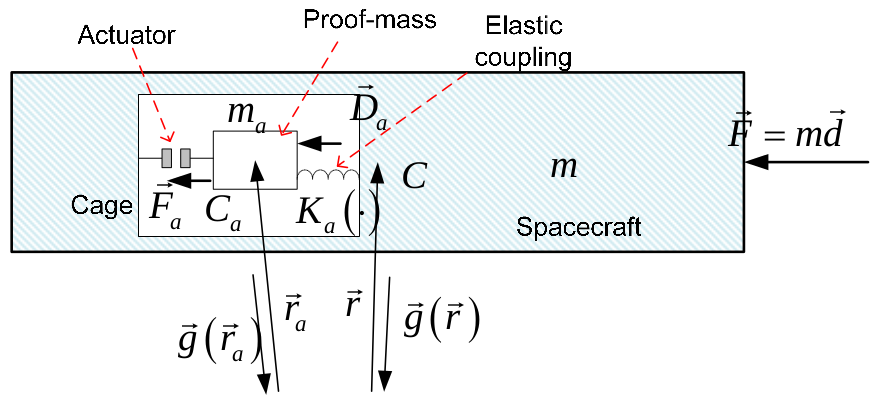
\includegraphics[width=\textwidth]{modelling/attitude_kinematics_and_dynamics/image/accelerometro.png}
  \caption{Massa di prova di un accelerometro}
  \label{fig:accelerometro}
\end{center}
\end{figure}
Indichiamo con $m$ la massa del satellite e con $m_a$ la massa della proof-mass,
$\vec{r}$ e $\vec{v}$ indicano la posizione  e la velocità del satellite, mentre
$\vec{r}_a$ e $\vec{v}_a$ indicano la posizione e la velocità della massa di
prova. Le equazioni di Newton della massa $m_a$ e del satellite sono
\begin{equation}
\dot{\vec{v}}(t)=-\vec{g}(\vec{r}(t))+\frac{\vec{F}(t)-\vec{F}_a(t)}{m}
\end{equation}
\begin{equation}
\dot{\vec{v}}_a(t)=-\vec{g}(\vec{r}_a(t))+\frac{\vec{F}_a(t)}{m_a}+\frac{\vec{D}_a(t)}{m_a}
\end{equation}
dove $\vec{D}_a$ indica le forze parassite agenti sulla proof-mass. Attraverso
la misura di $\vec{F}_a$ è quindi possibile risalire alle forze esterne al
satellite.

Tra gli errori di misura che affliggono le misurazioni effettuate tramite un accelerometro
è presente il bias, cioè un offset sistematico, dovuto alla tecnologia costruttiva, che viene
aggiunto alle misure. Nel controllo, purtroppo, tale errore viene interpretato come disturbo
dall’osservatore che quindi stima il drag sommato alla polarizzazione dell’accelerometro. Per
ovviare a tale difetto si agisce eliminando il valor medio del bias dall’uscita dell’osservatore.
Tuttavia l’orbita non sarà mai priva di accelerazioni non gravitazionali, poiché tra gli errori
dell’accelerometro è presente anche una deriva aleatoria.
\subsection{Perturbations}
L'interazione del satellite con l'ambiente circostante genera coppie che ne
disturbano l'assetto. Le principali perturbazioni sono:
\begin{description}
\item[Gradiente di gravità] generato dalla non uniformità del campo
gravitazionale terrestre, causa coppie disturbanti soprattutto a orbite basse
\item[Radiazioni elettromagnetiche] provenienti dal Sole e dagli altri pianeti,
queste onde urtano il satellite alterandone l'assetto
\item[Forze aerodinamiche] particelle esterne, dovute all'atmosfera terrestre,
colpiscono la superficie del satellite causando una pressione e quindi forze e
coppie che disturbano sia l'orbita che l'assetto
\item[Campo magnetico terrestre] interagisce con il dipolo elettrico del
satellite generato dalla strumentazione elettronica
\end{description}

Le coppie generate dall'interazione col gradiente gravitazionale terrestre sono
dovute alla non uniformità della distribuzione di massa della Terra e dalla
sua non sfericità, infatti l'accelerazione gravitazionale terrestre risulta
essere in funzione della distanza $\vec{r}$ dal centro della Terra
\begin{equation}
|\vec{g}(\vec{r}_c)|\approx9.81 [m/s^2], \ \vec{r}_c=R_E
\end{equation}
dove $R_E$ è la misura del raggio equatoriale della Terra.
Indicando con $\vec{s}$ la posizione di un generico punto del satellite rispetto
al centro di massa di quest'ultimo, possiamo calcolare la coppia di gravità
\begin{equation}
{\bf M}_g(t)=\int_V\vec{s}\times\vec{g}(\vec{r})dm
\end{equation}
sviluppando il vettore accelerazione gravitazionale, si ottiene
\begin{equation}
{\bf M}_g(t)=\int_V\vec{s}\times U_b({\bf r}_c){\bf s}dm
\label{eq:coppia_gravita}
\end{equation}
dove $U_b({\bf r}_c)$ è la matrice del gradiente di gravità nelle coordinate
corpo. Se gli assi corpo coincidono con gli assi principali di inerza,
l'equazione \ref{eq:coppia_gravita} diventa
\begin{equation}
{\bf M}_g(t)=\int_V 
\begin{bmatrix}
0 & -s_3 & s_2 \\
s_3 & 0 & -s_1 \\
-s_2 & s_1 & 0
\end{bmatrix}
[U_b]\begin{bmatrix}
s_1 \\ s_2 \\ s_3
\end{bmatrix} dm,
\end{equation}
con
\[ U_b=
\begin{bmatrix}
(J_3-J_2)U_{23} \\ (J_1-J_3)U_{13} \\ (J_2-J_1)U_{12}
\end{bmatrix}
\]
da cui si deduce che in caso di simmetria sferica ${\bf M}_g=0$

Per semplificare i calcoli ipotizziamo una gravità sferica, sotto questa ipotesi
possiamo scrivere
\begin{equation}
{\bf g}({\bf r}_c)=-\left(\frac{\mu_E}{r_c^3}\right){\bf r}_c
\end{equation}
dove $\mu_E=Gm_E$, adesso ricalcoliamo il tensore di gravità, che descrive come
varia nello spazio l’accelerazione di gravità dovuta ad un gravità sferica.
\begin{equation}
{\bf M}_g(t)=\int_V\vec{s}\times U_b({\bf r}_c){\bf s} \ dm=\frac{3\mu_E}{r_c^5}
\begin{bmatrix}
(J_3-J_2)y_cz_c \\ (J_1-J-3)x_cz_c \\ (J_2-J_1)x_cy_c
\end{bmatrix}
\end{equation}
Il che dimostra come in caso di simmetria cilindrica, la terza componente non
appare. Inoltre la coppia del gradiente gravità risulta essere ortogonale alla
verticale locale $\bar{r}_c$ e diminuisce col cubo della distanza dal satellite
al centro di massa del pianeta.
\subsection{Simulated runs without control}
Nello stesso modo con cui abbiamo realizzato la simulazione per lo studio
dell'orbita, lanciamo la simulazione con i parametri settati nel seguente modo
\begin{lstlisting}[language=matlab,breaklines=true]
GravityTypeFlag=1;		%(1=J2 Gravity Model/=0 Spherical)
GravityGradientTorqueFlag=1;	%1=Gravity Gradient Torque ON/0=OFF 
DragForceDisturbancesFlag=1;	%0=Drag Force Disturbance OFF/1=OFF
DragTorquesDisturbancesFlag=1;	%0=Drag Torque Disturbance OFF/1=ON
DragFreeControlFlag=0;		%0=Drag Free Control OFF/1=ON
AttitudeControlFlag=0;		%0=Attitude Control OFF/1=ON
\end{lstlisting}
ovvero, il gradiente di gravità è non sferico, sono presenti le coppie di
disturbo dovute a quest'ultimo e i disturbi dovuti al drag, ma la simulazione
viene eseguita senza azionare alcun controllo.
Di seguito sono i riportati i plot dell'accelerazione dovuta al drag, della
stessa docuta al gradiente di gravità e il plot dell'assetto con i quaternioni.

\begin{SCfigure}[0.7][ht]
	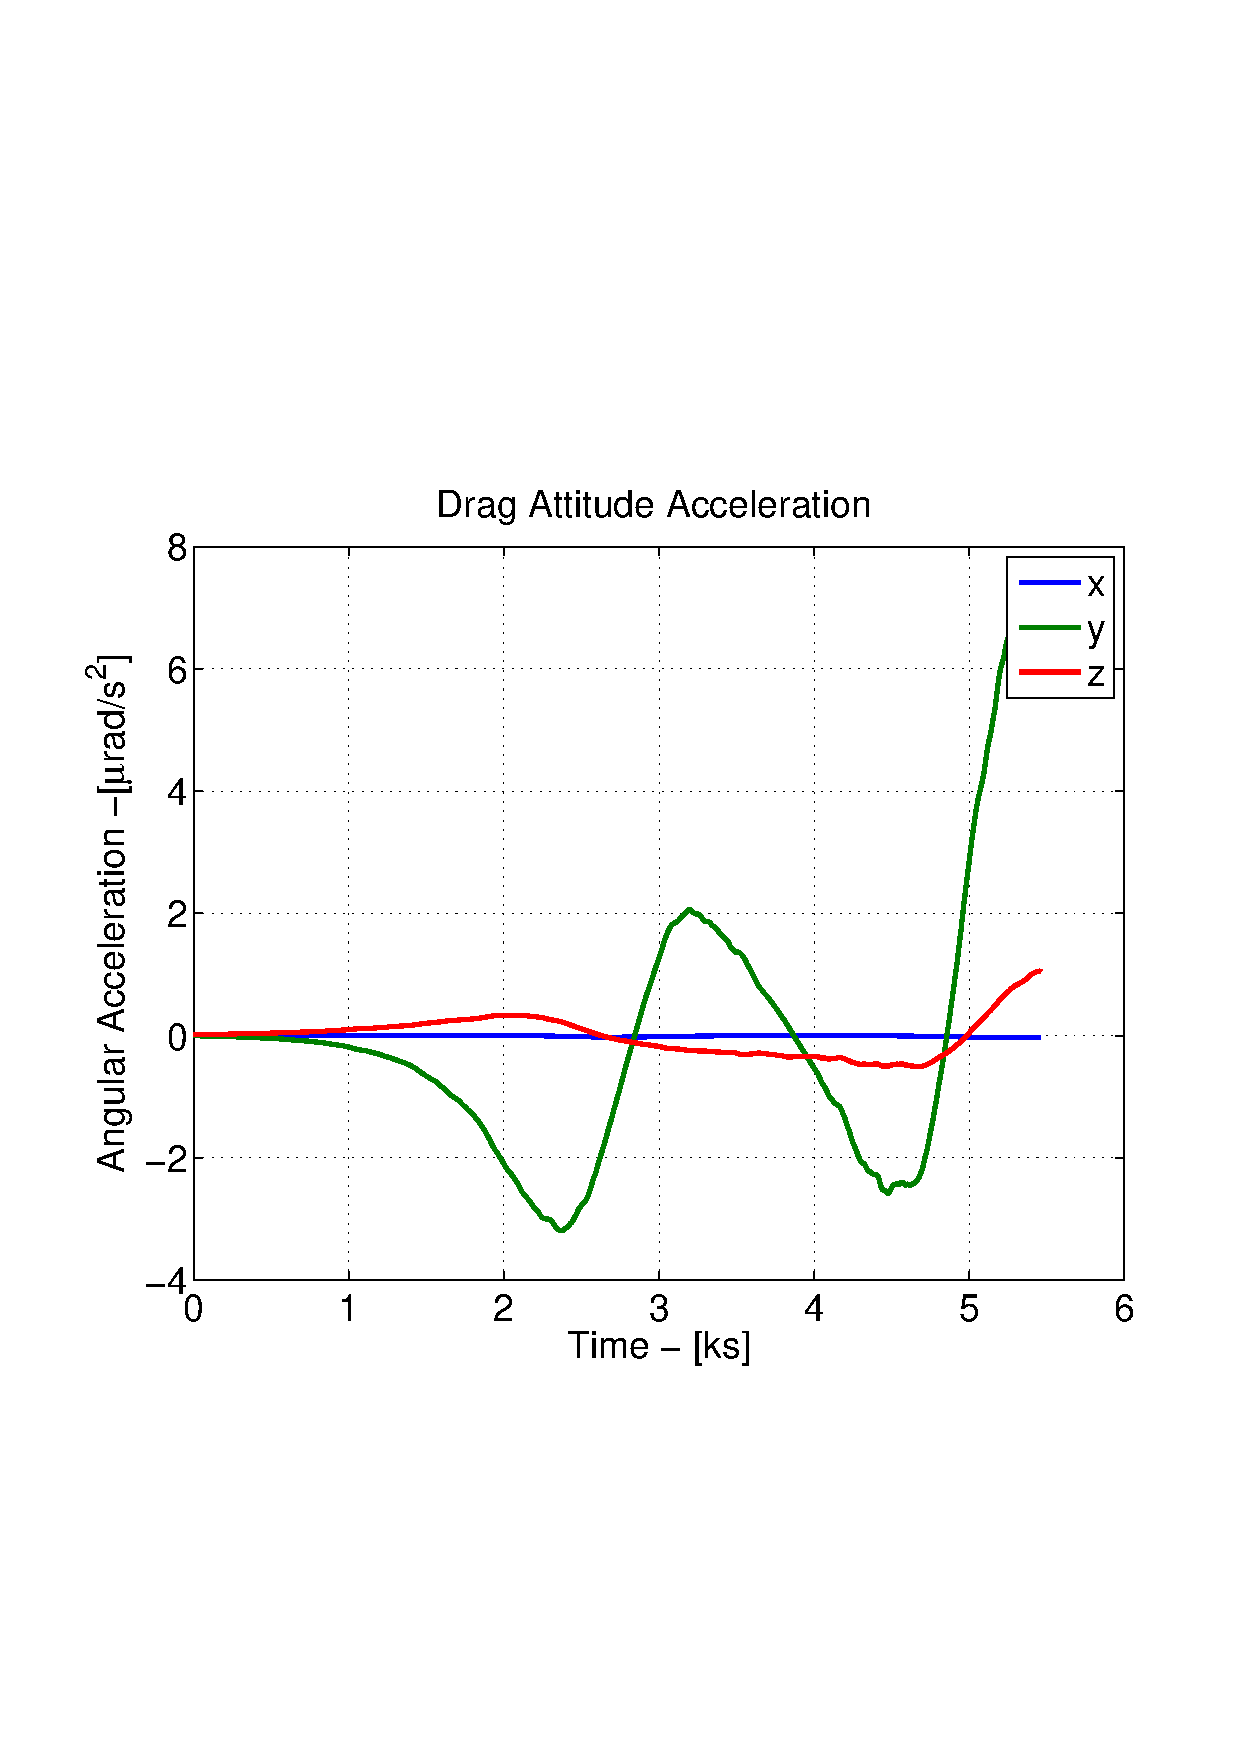
\includegraphics[width=.6\textwidth,clip=true,trim=1cm
	6cm
	1cm
	8cm]{modelling/attitude_kinematics_and_dynamics/image/DragAttitudeAcceleration.pdf}
	\caption{\emph{Accelerazione dovuta al drag} espressa nel riferimento corpo}
	\label{fig:drag-acceleration}
\end{SCfigure}

\begin{SCfigure}[0.7][ht]
	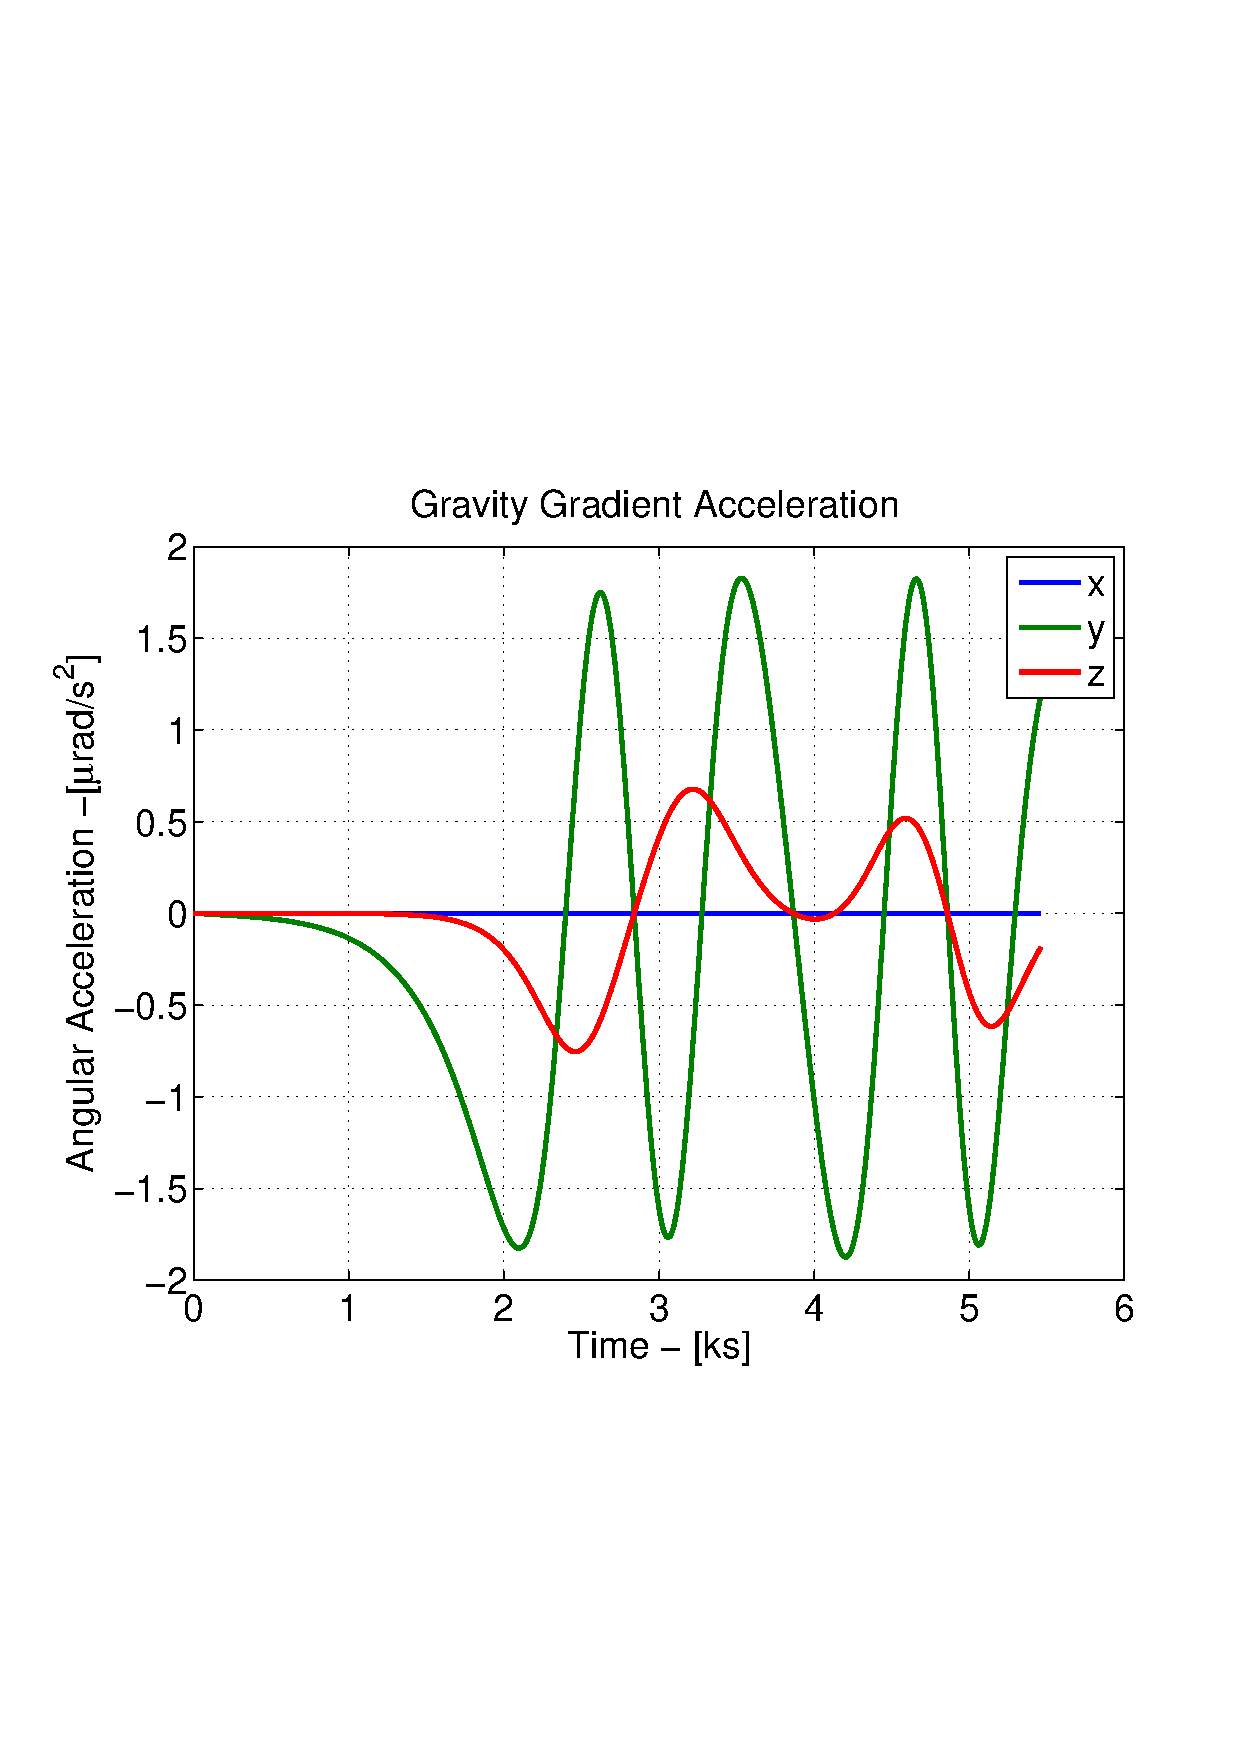
\includegraphics[width=.6\textwidth,clip=true,trim=1cm
	6cm
	1cm
	8cm]{modelling/attitude_kinematics_and_dynamics/image/GravityGradientAcceleration.pdf}
	\caption{\emph{Accelerazione dovuta gradiente di gravità} espressa nel
	riferimento corpo, le variazioni sono dovute all'appiattimento ai poli del
	globo terrestre}
	\label{fig:gravity-acceleration}
\end{SCfigure}

\begin{SCfigure}[0.7][ht]
	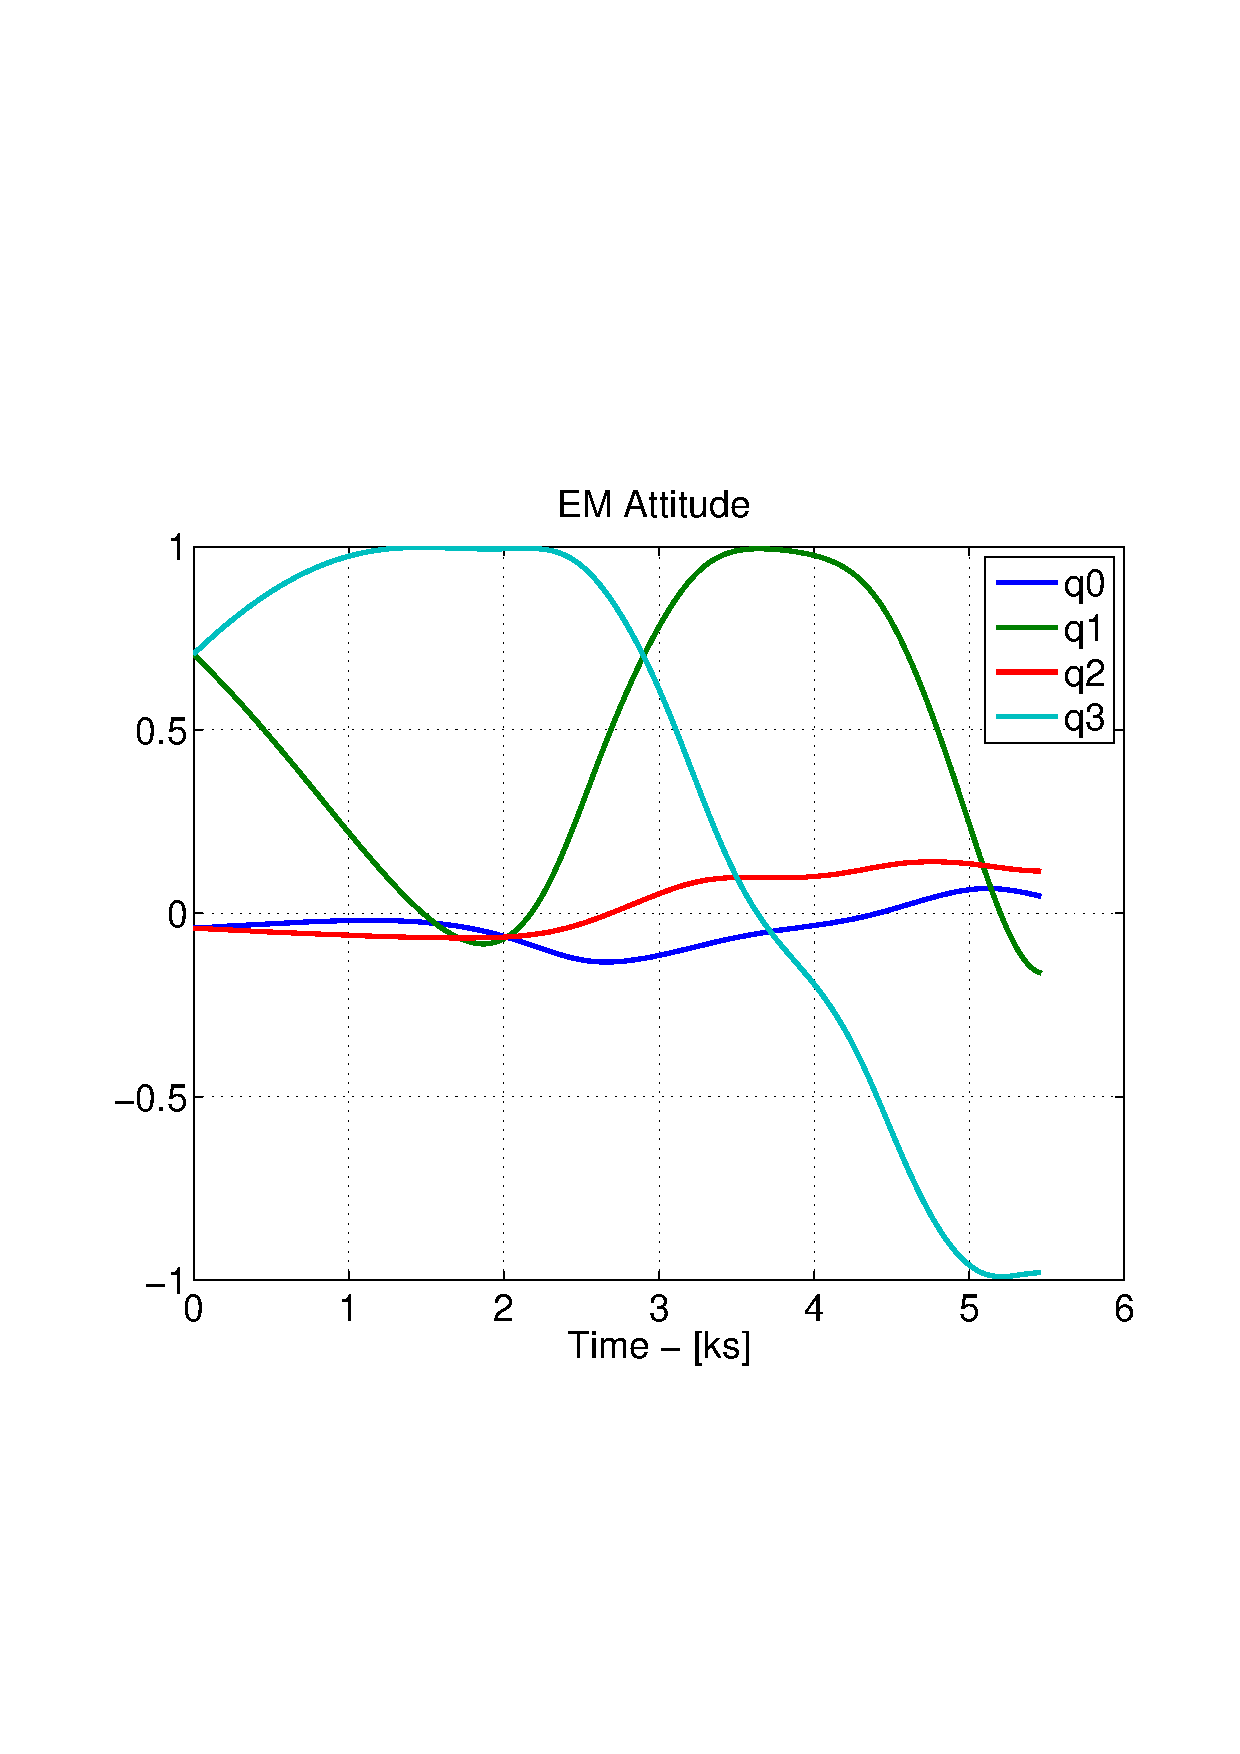
\includegraphics[width=.6\textwidth,clip=true,trim=1cm
	6cm
	1cm
	8cm]{modelling/attitude_kinematics_and_dynamics/image/EMAttitude.pdf}
	\caption{\emph{Assetto} in uscita dall'Embedded Model ed  espresso attraverso
	i quaternioni}
	\label{fig:attitude}
\end{SCfigure}
%###
\end{section}